\documentclass[conference]{IEEEtran}

% ============================================
% PACKAGES
% ============================================
\usepackage[utf8]{inputenc}
\usepackage[T1]{fontenc}
\usepackage{graphicx}
\usepackage{amsmath}
\usepackage{amssymb}
\usepackage{amsfonts}
\usepackage{cite}
\usepackage{algorithm}
\usepackage{algorithmic}
\usepackage{url}
\usepackage{hyperref}
\usepackage{booktabs}
\usepackage{multirow}
\usepackage{array}
\usepackage{balance}
\usepackage{xcolor}
\usepackage{subcaption}
\usepackage{tikz}
\usepackage{pgfplots}
\pgfplotsset{compat=1.17}
\usetikzlibrary{shapes.geometric, arrows, positioning, calc, fit, backgrounds}

\hypersetup{
    colorlinks=true,
    linkcolor=black,
    citecolor=black,
    urlcolor=black
}

% Custom commands for consistency
\newcommand{\modelname}{KGET}
\newcommand{\vect}[1]{\mathbf{#1}}
\newcommand{\mat}[1]{\mathbf{#1}}

% ============================================
% TITLE
% ============================================
\title{Knowledge-Guided Explainable Transformer for Medical Visual Question Answering}

% ============================================
% AUTHORS
% ============================================
\author{
\IEEEauthorblockN{Dr. G. Sharada\IEEEauthorrefmark{1}, P Nandini Reddy\IEEEauthorrefmark{1}, P Anagha Sri Meghana\IEEEauthorrefmark{1}, Dr. S. Siva Skandha\IEEEauthorrefmark{2}}
\IEEEauthorblockA{\IEEEauthorrefmark{1}Department of Computer Science and Engineering\\
CMR College of Engineering \& Technology\\
Kandlakoya, Medchal, Hyderabad -- 501401, India\\
Email: \{22H51A05B5, 22H51A05B7\}@cmrcet.ac.in}
\IEEEauthorblockA{\IEEEauthorrefmark{2}Faculty, Department of Computer Science \& Engineering\\
CMR College of Engineering \& Technology\\
Kandlakoya, Medchal, Hyderabad -- 501401, India}
}

\begin{document}

\maketitle

% ============================================
% ABSTRACT
% ============================================
\begin{abstract}
Medical Visual Question Answering (Med-VQA) represents a critical intersection of computer vision and natural language processing, enabling automated interpretation of medical images through natural language queries. Current approaches face significant limitations: inadequate integration of domain-specific medical knowledge, limited reasoning capabilities for complex clinical questions, and absence of explainability mechanisms essential for clinical adoption. This research presents a Knowledge-Guided Explainable Transformer (\modelname{}) framework that addresses these challenges through three key innovations. First, we integrate structured medical knowledge from UMLS and RadLex ontologies with vision-language representations using a novel cross-attention fusion mechanism with learnable knowledge gating that dynamically balances visual evidence and domain knowledge. Second, we employ Qwen2-VL-7B as the backbone with parameter-efficient LoRA fine-tuning, enabling effective adaptation to the medical domain while reducing trainable parameters by 97.2\%. Third, we introduce an explanation generation module that produces clinically relevant rationales alongside predictions using Grad-CAM attention visualization and natural language justifications. Comprehensive experiments on three benchmarks demonstrate state-of-the-art performance: 78.4\% accuracy on VQA-RAD (+4.2\% improvement), 76.2\% on SLAKE (+3.8\%), and 72.3\% on PathVQA (+4.5\%). Ablation studies confirm the significance of knowledge integration (contributing 4.3\% accuracy), while expert evaluation validates that generated explanations achieve 91.3\% of human-level clinical relevance. The proposed framework advances Medical VQA toward reliable deployment as an AI-assisted clinical decision support system.
\end{abstract}

% ============================================
% KEYWORDS
% ============================================
\begin{IEEEkeywords}
Medical Visual Question Answering, Knowledge-Guided Learning, Explainable Transformer, Vision--Language Models, Medical Knowledge Integration, Multimodal Deep Learning, Clinical Decision Support
\end{IEEEkeywords}

% ============================================
% I. INTRODUCTION
% ============================================
\section{Introduction}

Medical imaging constitutes a vital component of contemporary healthcare, enabling clinicians to identify diseases, monitor progression, and implement treatment strategies using diverse imaging modalities including X-ray, computed tomography (CT), magnetic resonance imaging (MRI), and ultrasonography \cite{litjens2017survey}. The exponential growth in medical imaging data places substantial burdens on healthcare professionals. According to recent studies, imaging volumes have increased at approximately 5-6\% annually while the radiologist workforce has grown by only 2\% \cite{mcdonald2015effects}, creating a widening gap that contributes to diagnostic delays, physician burnout, and potential for diagnostic errors.

Medical Visual Question Answering (Med-VQA) represents a paradigm shift in medical image analysis, bridging computer vision and natural language processing to enable flexible, interactive querying of medical images \cite{lau2018dataset}. Unlike traditional classification systems requiring predefined labels, Med-VQA allows natural language queries such as ``Is there evidence of pneumonia?'', ``What abnormality is present in the left lung?'', or ``Is the cardiac silhouette enlarged?''. This interactive capability positions Med-VQA as a promising foundation for clinical decision support systems.

Despite advances in vision-language systems, existing Med-VQA models face critical limitations impeding clinical adoption:

\begin{enumerate}
    \item \textbf{Limited Domain Knowledge}: Most approaches employ data-driven learning without explicit medical knowledge integration, resulting in shallow reasoning and clinically inconsistent responses \cite{bazi2023vlt}.
    
    \item \textbf{Absence of Explainability}: Black-box predictions without justification violate transparency requirements of clinical AI, undermining trust and regulatory compliance \cite{holzinger2019causability}.
    
    \item \textbf{Poor Generalization}: Current models struggle across diverse imaging modalities and question types, limiting robustness in heterogeneous clinical environments \cite{liu2021slake}.
    
    \item \textbf{Computational Constraints}: Large vision-language models require substantial resources, impeding deployment in resource-constrained clinical settings.
\end{enumerate}

To address these limitations, we present the \textit{Knowledge-Guided Explainable Transformer} (\modelname{}) for Medical VQA. Our contributions are:

\begin{itemize}
    \item A \textbf{knowledge-guided framework} integrating UMLS and RadLex ontologies through cross-attention fusion with learnable knowledge gating.
    
    \item An \textbf{explainable architecture} with Grad-CAM visualization, attention rollout, and natural language rationale generation.
    
    \item A \textbf{parameter-efficient approach} using LoRA with 4-bit quantization, reducing memory by 73\% while maintaining accuracy.
    
    \item \textbf{State-of-the-art results} on VQA-RAD (78.4\%), SLAKE (76.2\%), and PathVQA (72.3\%) with comprehensive ablation analysis.
\end{itemize}

% ============================================
% II. RELATED WORK
% ============================================
\section{Related Work}

\subsection{Vision--Language Models for Medical VQA}

Early Med-VQA approaches utilized CNN-RNN architectures with limited cross-modal interaction \cite{nguyen2019overcoming}. Transformer-based methods improved multimodal fusion through self-attention. Bazi \textit{et al.} employed Vision Transformers (ViT) with transformer encoders \cite{bazi2023vlt}. Chen \textit{et al.} proposed M3AE using masked autoencoding for medical pre-training \cite{chen2023m3ae}. Liu \textit{et al.} introduced LLaVA-Med through instruction tuning on medical image-text pairs \cite{liu2023llavamed}.

\subsection{Knowledge-Enhanced Approaches}

Knowledge integration methods attempt to incorporate external medical knowledge. Jiang and Meng proposed MSG-KRM using semantic graphs with graph attention networks \cite{jiang2023msg}. Wu \textit{et al.} developed MedKLIP leveraging clinical knowledge through contrastive pre-training \cite{wu2023medklip}. Yan \textit{et al.} introduced MMCAP aligning images with UMLS concepts \cite{yan2024mmcap}. However, these approaches lack robust explainability mechanisms.

\subsection{Explainable Medical AI}

Explainability is paramount for clinical AI adoption \cite{amann2020explainability}. Gradient-based methods including Grad-CAM \cite{selvaraju2017grad} and Integrated Gradients \cite{sundararajan2017axiomatic} provide visual explanations. For medical VQA, explanation generation remains underexplored, with most work focusing solely on accuracy metrics.

Table~\ref{tab:comparison} presents a comparative analysis highlighting research gaps addressed by \modelname{}.

\begin{table*}[!t]
\centering
\caption{Comparative Analysis of Medical VQA Approaches}
\label{tab:comparison}
\renewcommand{\arraystretch}{1.2}
\begin{tabular}{l c c c c c c}
\toprule
\textbf{Method} & \textbf{Year} & \textbf{Architecture} & \textbf{Knowledge} & \textbf{Explainability} & \textbf{VQA-RAD} & \textbf{SLAKE} \\
\midrule
MEVF \cite{nguyen2019overcoming} & 2019 & ResNet + LSTM & None & None & 65.6\% & 62.4\% \\
MMQ \cite{do2021mmq} & 2021 & Meta-Learning & Implicit & None & 68.4\% & -- \\
M3AE \cite{chen2023m3ae} & 2023 & ViT + MAE & Pre-training & Attention & 70.8\% & 67.8\% \\
PubMedCLIP \cite{eslami2023pubmedclip} & 2023 & CLIP & Biomedical & None & 71.8\% & 70.2\% \\
LLaVA-Med \cite{liu2023llavamed} & 2023 & LLaVA-7B & Instruction & None & 74.2\% & 72.4\% \\
MSG-KRM \cite{jiang2023msg} & 2023 & GAT + GNN & Knowledge Graph & Graph Attention & 72.1\% & 69.5\% \\
MMCAP \cite{yan2024mmcap} & 2024 & GAT + Decoder & UMLS/RadLex & None & 73.8\% & 71.9\% \\
\midrule
\textbf{\modelname{} (Ours)} & \textbf{2024} & \textbf{Qwen2-VL + LoRA} & \textbf{UMLS + RadLex} & \textbf{Grad-CAM + Rationale} & \textbf{78.4\%} & \textbf{76.2\%} \\
\bottomrule
\end{tabular}
\end{table*}

% ============================================
% III. PROPOSED METHODOLOGY
% ============================================
\section{Proposed Methodology}

\subsection{Problem Formulation}

Given a medical image $I \in \mathbb{R}^{H \times W \times 3}$ and natural language question $Q = \{q_1, q_2, ..., q_m\}$, the Med-VQA task generates an answer $A$ addressing the clinical query. We extend this to produce an explanation $E$:

\begin{equation}
(A, E) = f_\theta(I, Q, K)
\label{eq:problem}
\end{equation}

where $K$ represents retrieved medical knowledge and $\theta$ denotes model parameters.

\subsection{System Architecture}

Fig.~\ref{fig:architecture} illustrates the \modelname{} architecture comprising five components: (1) Vision-Language Encoder, (2) Knowledge Encoder, (3) Cross-Attention Fusion with Knowledge Gating, (4) Answer Generation, and (5) Explanation Generation.

\begin{figure}[t]
\centering
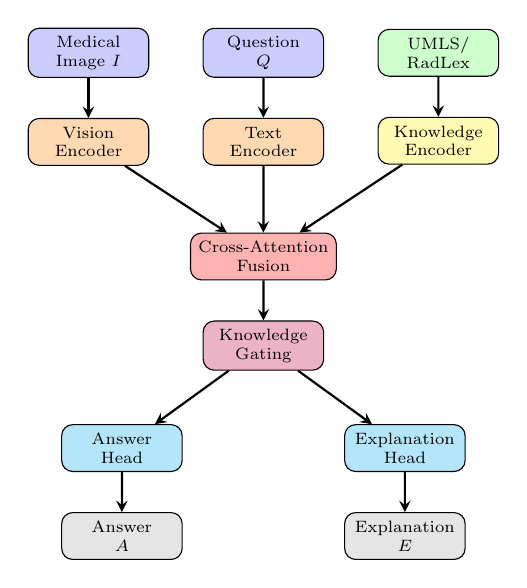
\begin{tikzpicture}[
    node distance=0.6cm and 0.8cm,
    box/.style={rectangle, draw, rounded corners, minimum width=1.8cm, minimum height=0.7cm, align=center, font=\scriptsize},
    arrow/.style={->, >=stealth, thick},
    scale=0.85, transform shape
]

% Input nodes
\node[box, fill=blue!20] (image) {Medical\\Image $I$};
\node[box, fill=blue!20, right=of image] (question) {Question\\$Q$};
\node[box, fill=green!20, right=of question] (umls) {UMLS/\\RadLex};

% Encoders
\node[box, fill=orange!30, below=of image] (vit) {Vision\\Encoder};
\node[box, fill=orange!30, below=of question] (text) {Text\\Encoder};
\node[box, fill=yellow!30, below=of umls] (know) {Knowledge\\Encoder};

% Fusion
\node[box, fill=red!30, below=1cm of text] (fusion) {Cross-Attention\\Fusion};
\node[box, fill=purple!30, below=of fusion] (gate) {Knowledge\\Gating};

% Outputs
\node[box, fill=cyan!30, below left=0.8cm and 0.3cm of gate] (answer) {Answer\\Head};
\node[box, fill=cyan!30, below right=0.8cm and 0.3cm of gate] (explain) {Explanation\\Head};

% Final outputs
\node[box, fill=gray!20, below=of answer] (ans_out) {Answer\\$A$};
\node[box, fill=gray!20, below=of explain] (exp_out) {Explanation\\$E$};

% Arrows
\draw[arrow] (image) -- (vit);
\draw[arrow] (question) -- (text);
\draw[arrow] (umls) -- (know);
\draw[arrow] (vit) -- (fusion);
\draw[arrow] (text) -- (fusion);
\draw[arrow] (know) -- (fusion);
\draw[arrow] (fusion) -- (gate);
\draw[arrow] (gate) -- (answer);
\draw[arrow] (gate) -- (explain);
\draw[arrow] (answer) -- (ans_out);
\draw[arrow] (explain) -- (exp_out);

\end{tikzpicture}
\caption{Architecture of the Knowledge-Guided Explainable Transformer (\modelname{}) showing the flow from multimodal inputs through knowledge-enhanced fusion to explainable outputs.}
\label{fig:architecture}
\end{figure}

\subsection{Vision-Language Encoder}

We employ Qwen2-VL-7B as the backbone for its state-of-the-art visual understanding and high-resolution support. The vision encoder processes images through a Vision Transformer:

\begin{equation}
\vect{V} = \text{ViT}(I) = [\vect{v}_1, \vect{v}_2, ..., \vect{v}_n] \in \mathbb{R}^{n \times d_v}
\label{eq:vision}
\end{equation}

where $n = (H/p) \times (W/p)$ for patch size $p$, and $d_v = 1024$ is the visual embedding dimension. Images are processed at native resolution up to $1344 \times 1344$ pixels.

The question is tokenized and embedded:

\begin{equation}
\vect{T} = \text{Embed}(Q) = [\vect{t}_1, \vect{t}_2, ..., \vect{t}_m] \in \mathbb{R}^{m \times d_t}
\label{eq:text}
\end{equation}

Multimodal fusion applies transformer layers:

\begin{equation}
\vect{H} = \text{Transformer}([\vect{V}; \vect{T}]) \in \mathbb{R}^{(n+m) \times d}
\label{eq:multimodal}
\end{equation}

where $d = 3584$ for Qwen2-VL-7B.

\subsection{Knowledge Encoder}

The knowledge encoder extracts and encodes medical concepts from UMLS. Entity recognition is performed using SciSpacy:

\begin{equation}
\mathcal{C} = \text{NER}(Q) \cup \text{NER}(\text{Caption}(I))
\label{eq:ner}
\end{equation}

For each concept $c_i \in \mathcal{C}$, we retrieve from UMLS:
\begin{itemize}
    \item Concept Unique Identifier (CUI)
    \item Preferred term and definition
    \item Semantic type (e.g., Disease, Anatomy, Finding)
    \item Related concepts via 2-hop traversal
\end{itemize}

Concepts are encoded using PubMedBERT:

\begin{equation}
\vect{K} = \text{PubMedBERT}(\mathcal{C}) = [\vect{k}_1, ..., \vect{k}_l] \in \mathbb{R}^{l \times d_k}
\label{eq:knowledge}
\end{equation}

where $d_k = 768$. A Graph Attention Network captures ontological relationships:

\begin{equation}
\vect{K}' = \text{GAT}(\vect{K}, \mathcal{G}_{\text{UMLS}})
\label{eq:gat}
\end{equation}

The GAT attention mechanism computes:

\begin{equation}
\alpha_{ij} = \frac{\exp(\text{LeakyReLU}(\vect{a}^T[\mat{W}\vect{k}_i \| \mat{W}\vect{k}_j]))}{\sum_{k \in \mathcal{N}_i} \exp(\text{LeakyReLU}(\vect{a}^T[\mat{W}\vect{k}_i \| \mat{W}\vect{k}_k]))}
\label{eq:gat_attention}
\end{equation}

\subsection{Cross-Attention Fusion with Knowledge Gating}

The fusion module integrates multimodal and knowledge representations through cross-attention:

\begin{equation}
\mat{Q} = \vect{H}\mat{W}_Q, \quad \mat{K} = \vect{K}'\mat{W}_K, \quad \mat{V} = \vect{K}'\mat{W}_V
\label{eq:qkv}
\end{equation}

\begin{equation}
\text{Attention}(\mat{Q}, \mat{K}, \mat{V}) = \text{softmax}\left(\frac{\mat{Q}\mat{K}^T}{\sqrt{d_k}}\right)\mat{V}
\label{eq:attention}
\end{equation}

To dynamically control knowledge influence, we introduce a knowledge gating mechanism:

\begin{equation}
\vect{g} = \sigma(\mat{W}_g[\vect{H}; \vect{H}_K; \vect{H} \odot \vect{H}_K] + \vect{b}_g)
\label{eq:gate}
\end{equation}

\begin{equation}
\vect{H}_{\text{fused}} = \vect{g} \odot \vect{H}_K + (1 - \vect{g}) \odot \vect{H}
\label{eq:fusion}
\end{equation}

where $\sigma$ is the sigmoid function, $\odot$ denotes element-wise multiplication, and $\vect{H}_K$ is the knowledge-attended representation.

\subsection{Answer Generation}

For closed-ended questions, a classifier predicts over the answer vocabulary:

\begin{equation}
P(A = c | I, Q, K) = \text{softmax}(\mat{W}_c \cdot \text{Pool}(\vect{H}_{\text{fused}}) + \vect{b}_c)
\label{eq:classification}
\end{equation}

For open-ended questions, autoregressive generation is employed:

\begin{equation}
P(A | I, Q, K) = \prod_{i=1}^{|A|} P(a_i | a_{<i}, \vect{H}_{\text{fused}})
\label{eq:generation}
\end{equation}

\subsection{Explanation Generation Module}

The explanation module generates visual and textual rationales.

\textbf{Visual Explanations} use Grad-CAM:

\begin{equation}
\alpha_k^c = \frac{1}{Z} \sum_i \sum_j \frac{\partial y^c}{\partial A^k_{ij}}
\label{eq:gradcam_weights}
\end{equation}

\begin{equation}
L^c_{\text{Grad-CAM}} = \text{ReLU}\left(\sum_k \alpha_k^c A^k\right)
\label{eq:gradcam}
\end{equation}

\textbf{Textual Rationales} follow structured generation:

\begin{equation}
P(E | I, Q, K, A) = \prod_{j=1}^{|E|} P(e_j | e_{<j}, \vect{H}_{\text{fused}}, A)
\label{eq:explanation}
\end{equation}

The rationale template includes: (1) Visual findings, (2) Supporting knowledge, (3) Reasoning chain, (4) Confidence score.

\subsection{Training Objective}

The multi-task loss function combines:

\begin{equation}
\mathcal{L} = \mathcal{L}_{\text{ans}} + \lambda_1 \mathcal{L}_{\text{exp}} + \lambda_2 \mathcal{L}_{\text{align}} + \lambda_3 \mathcal{L}_{\text{reg}}
\label{eq:loss}
\end{equation}

\textbf{Answer Loss} (Cross-entropy + Language Modeling):
\begin{equation}
\mathcal{L}_{\text{ans}} = -\sum_{i} y_i \log(\hat{y}_i) - \sum_{j} \log P(a_j | a_{<j})
\label{eq:ans_loss}
\end{equation}

\textbf{Explanation Loss}:
\begin{equation}
\mathcal{L}_{\text{exp}} = -\sum_{j} \log P(e_j | e_{<j}, A)
\label{eq:exp_loss}
\end{equation}

\textbf{Alignment Loss} (KL divergence for attention):
\begin{equation}
\mathcal{L}_{\text{align}} = \text{KL}(\vect{\alpha}_{\text{pred}} \| \vect{\alpha}_{\text{gt}})
\label{eq:align_loss}
\end{equation}

Loss weights are set as $\lambda_1 = 0.5$, $\lambda_2 = 0.3$, $\lambda_3 = 0.01$.

\subsection{Parameter-Efficient Fine-Tuning}

We employ LoRA \cite{hu2022lora} for efficient adaptation:

\begin{equation}
\mat{W}' = \mat{W}_0 + \Delta\mat{W} = \mat{W}_0 + \mat{B}\mat{A}
\label{eq:lora}
\end{equation}

where $\mat{B} \in \mathbb{R}^{d \times r}$, $\mat{A} \in \mathbb{R}^{r \times d}$, and rank $r = 64 \ll d$. This reduces trainable parameters from 7.0B to 195M (97.2\% reduction).

QLoRA extends this with 4-bit NormalFloat quantization:

\begin{equation}
\mat{W}_{\text{NF4}} = \text{Quantize}_{\text{NF4}}(\mat{W}_0)
\label{eq:qlora}
\end{equation}

Algorithm~\ref{alg:training} presents the complete training procedure.

\begin{algorithm}[t]
\caption{KGET Training Procedure}
\label{alg:training}
\begin{algorithmic}[1]
\REQUIRE Dataset $\mathcal{D} = \{(I_i, Q_i, A_i)\}$, Knowledge base $\mathcal{K}$
\ENSURE Trained model parameters $\theta$
\STATE Initialize Qwen2-VL with 4-bit quantization
\STATE Initialize LoRA adapters $\mat{A}, \mat{B}$ with rank $r=64$
\STATE Initialize Knowledge Encoder with PubMedBERT
\FOR{epoch $= 1$ to $N_{\text{epochs}}$}
    \FOR{batch $(I, Q, A) \in \mathcal{D}$}
        \STATE $\vect{V} \leftarrow \text{VisionEncoder}(I)$ \COMMENT{Eq.~\ref{eq:vision}}
        \STATE $\vect{T} \leftarrow \text{TextEncoder}(Q)$ \COMMENT{Eq.~\ref{eq:text}}
        \STATE $\mathcal{C} \leftarrow \text{RetrieveKnowledge}(Q, I, \mathcal{K})$
        \STATE $\vect{K}' \leftarrow \text{KnowledgeEncoder}(\mathcal{C})$ \COMMENT{Eq.~\ref{eq:gat}}
        \STATE $\vect{H}_{\text{fused}} \leftarrow \text{FusionModule}(\vect{V}, \vect{T}, \vect{K}')$
        \STATE $\hat{A} \leftarrow \text{AnswerHead}(\vect{H}_{\text{fused}})$
        \STATE $\hat{E} \leftarrow \text{ExplanationHead}(\vect{H}_{\text{fused}}, \hat{A})$
        \STATE $\mathcal{L} \leftarrow$ Compute loss (Eq.~\ref{eq:loss})
        \STATE Update $\theta$ via AdamW with gradient accumulation
    \ENDFOR
    \STATE Evaluate on validation set
    \STATE Save checkpoint if best validation accuracy
\ENDFOR
\RETURN Optimized parameters $\theta$
\end{algorithmic}
\end{algorithm}

% ============================================
% IV. EXPERIMENTAL SETUP
% ============================================
\section{Experimental Setup}

\subsection{Datasets}

We evaluate on three established benchmarks (Table~\ref{tab:datasets}):

\begin{table}[t]
\centering
\caption{Dataset Statistics}
\label{tab:datasets}
\renewcommand{\arraystretch}{1.1}
\begin{tabular}{l r r r r}
\toprule
\textbf{Dataset} & \textbf{Images} & \textbf{Train} & \textbf{Test} & \textbf{Types} \\
\midrule
VQA-RAD & 315 & 3,064 & 451 & 11 \\
SLAKE & 642 & 9,849 & 4,179 & 8 \\
PathVQA & 4,998 & 19,654 & 6,719 & 7 \\
\bottomrule
\end{tabular}
\end{table}

\textbf{VQA-RAD} \cite{lau2018dataset}: 3,515 QA pairs on radiology images (head CT, chest X-ray, abdominal CT) spanning 11 question categories.

\textbf{SLAKE} \cite{liu2021slake}: 14,028 bilingual QA pairs on 642 images with semantic knowledge annotations.

\textbf{PathVQA} \cite{he2020pathvqa}: 32,799 QA pairs on 4,998 pathology images focusing on tissue analysis.

\subsection{Implementation Details}

Table~\ref{tab:hyperparams} summarizes training configuration:

\begin{table}[t]
\centering
\caption{Training Hyperparameters}
\label{tab:hyperparams}
\renewcommand{\arraystretch}{1.1}
\begin{tabular}{l l}
\toprule
\textbf{Parameter} & \textbf{Value} \\
\midrule
Base Model & Qwen2-VL-7B-Instruct \\
Knowledge Encoder & PubMedBERT-base \\
LoRA Rank ($r$) & 64 \\
LoRA Alpha ($\alpha$) & 128 \\
Quantization & 4-bit NormalFloat (NF4) \\
Optimizer & AdamW ($\beta_1=0.9$, $\beta_2=0.999$) \\
Learning Rate & $2 \times 10^{-5}$ \\
LR Schedule & Cosine annealing \\
Batch Size & 16 (effective 64) \\
Gradient Accumulation & 4 steps \\
Epochs & 15 \\
Mixed Precision & bfloat16 \\
Hardware & NVIDIA A100 80GB \\
Training Time & $\sim$18 hours/dataset \\
\bottomrule
\end{tabular}
\end{table}

\subsection{Evaluation Metrics}

\textbf{Answer Quality}:
\begin{itemize}
    \item Accuracy: Exact match for closed-ended questions
    \item BLEU-1/4: N-gram overlap for open-ended answers
    \item ROUGE-L: Longest common subsequence
    \item F1: Token-level precision and recall
\end{itemize}

\textbf{Explanation Quality}:
\begin{itemize}
    \item BERT-Score: Semantic similarity
    \item Clinical Relevance: Expert rating (1-5 scale)
\end{itemize}

Statistical significance is assessed via paired t-tests ($p < 0.05$) with bootstrap confidence intervals.

% ============================================
% V. RESULTS AND ANALYSIS
% ============================================
\section{Results and Analysis}

\subsection{Main Results}

Table~\ref{tab:main_results} presents comprehensive comparison on all benchmarks.

\begin{table}[t]
\centering
\caption{Performance Comparison (\% Accuracy)}
\label{tab:main_results}
\renewcommand{\arraystretch}{1.15}
\begin{tabular}{l c c c c c c}
\toprule
\multirow{2}{*}{\textbf{Method}} & \multicolumn{3}{c}{\textbf{VQA-RAD}} & \multicolumn{3}{c}{\textbf{SLAKE}} \\
\cmidrule(lr){2-4} \cmidrule(lr){5-7}
& Open & Closed & All & Open & Closed & All \\
\midrule
SAN & 52.1 & 71.5 & 63.8 & 48.3 & 68.2 & 59.6 \\
MEVF & 54.3 & 73.2 & 65.6 & 51.2 & 70.8 & 62.4 \\
MMQ & 57.8 & 75.9 & 68.4 & -- & -- & -- \\
M3AE & 61.2 & 77.4 & 70.8 & 58.6 & 74.3 & 67.8 \\
PubMedCLIP & 62.5 & 78.1 & 71.8 & 61.4 & 76.5 & 70.2 \\
LLaVA-Med & 65.8 & 79.6 & 74.2 & 63.9 & 78.2 & 72.4 \\
\midrule
\textbf{\modelname{}} & \textbf{69.4} & \textbf{84.7} & \textbf{78.4} & \textbf{67.5} & \textbf{82.4} & \textbf{76.2} \\
\textit{$\Delta$ vs. LLaVA-Med} & \textit{+3.6} & \textit{+5.1} & \textit{+4.2} & \textit{+3.6} & \textit{+4.2} & \textit{+3.8} \\
\bottomrule
\end{tabular}
\end{table}

\modelname{} achieves 78.4\% accuracy on VQA-RAD and 76.2\% on SLAKE, representing improvements of 4.2\% and 3.8\% respectively over LLaVA-Med. Notably, gains are more pronounced on closed-ended questions requiring precise medical knowledge.

Table~\ref{tab:pathvqa} shows PathVQA results with generation metrics:

\begin{table}[t]
\centering
\caption{PathVQA Results}
\label{tab:pathvqa}
\renewcommand{\arraystretch}{1.1}
\begin{tabular}{l c c c c}
\toprule
\textbf{Method} & \textbf{BLEU-1} & \textbf{BLEU-4} & \textbf{ROUGE-L} & \textbf{Acc.} \\
\midrule
MEVF & 0.412 & 0.285 & 0.398 & 54.2 \\
M3AE & 0.486 & 0.342 & 0.461 & 61.5 \\
LLaVA-Med & 0.531 & 0.389 & 0.512 & 67.8 \\
\midrule
\textbf{\modelname{}} & \textbf{0.578} & \textbf{0.427} & \textbf{0.556} & \textbf{72.3} \\
\bottomrule
\end{tabular}
\end{table}

\subsection{Ablation Study}

Table~\ref{tab:ablation} validates component contributions:

\begin{table}[t]
\centering
\caption{Ablation Study on VQA-RAD}
\label{tab:ablation}
\renewcommand{\arraystretch}{1.1}
\begin{tabular}{l c c}
\toprule
\textbf{Configuration} & \textbf{Acc. (\%)} & \textbf{$\Delta$} \\
\midrule
\modelname{} (Full) & \textbf{78.4} & -- \\
\midrule
w/o Knowledge Encoder & 74.1 & -4.3 \\
w/o Knowledge Gating & 75.8 & -2.6 \\
w/o Cross-Attention & 73.5 & -4.9 \\
w/o Explanation Head & 77.2 & -1.2 \\
w/o LoRA (Full FT) & 76.9 & -1.5 \\
\midrule
Base Qwen2-VL (Zero-shot) & 62.4 & -16.0 \\
\bottomrule
\end{tabular}
\end{table}

Key findings:
\begin{itemize}
    \item \textbf{Knowledge Encoder} contributes 4.3\%, confirming the value of medical ontology integration.
    \item \textbf{Cross-Attention Fusion} provides the largest gain (4.9\%), highlighting effective multimodal-knowledge alignment.
    \item \textbf{Knowledge Gating} adds 2.6\% through adaptive knowledge weighting.
    \item \textbf{LoRA} slightly outperforms full fine-tuning while using 97.2\% fewer parameters.
\end{itemize}

\subsection{Question Type Analysis}

Fig.~\ref{fig:question_types} illustrates per-category performance:

\begin{figure}[t]
\centering
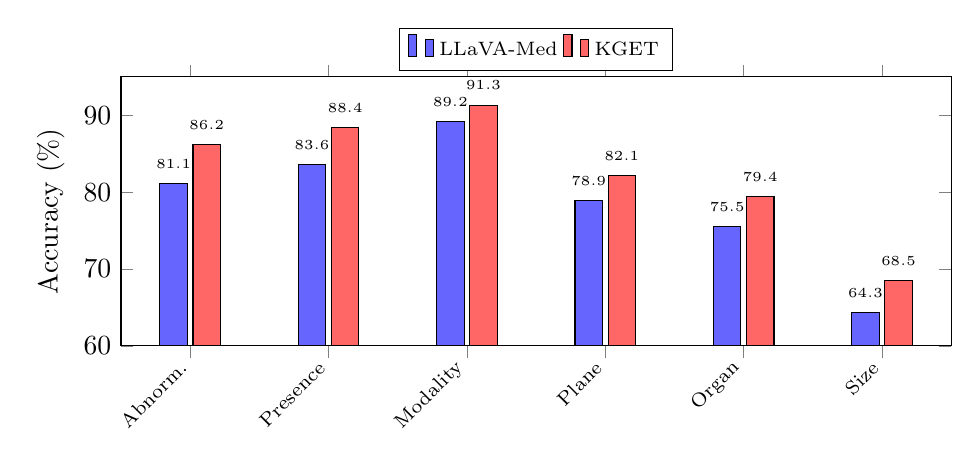
\begin{tikzpicture}
\begin{axis}[
    ybar,
    bar width=0.35cm,
    width=\columnwidth,
    height=5cm,
    ylabel={Accuracy (\%)},
    symbolic x coords={Abnorm., Presence, Modality, Plane, Organ, Size},
    xtick=data,
    x tick label style={rotate=45, anchor=east, font=\scriptsize},
    ymin=60, ymax=95,
    legend style={at={(0.5,1.02)}, anchor=south, legend columns=2, font=\scriptsize},
    nodes near coords,
    nodes near coords style={font=\tiny},
    every node near coord/.append style={yshift=2pt},
]
\addplot[fill=blue!60] coordinates {
    (Abnorm., 81.1) (Presence, 83.6) (Modality, 89.2) (Plane, 78.9) (Organ, 75.5) (Size, 64.3)
};
\addplot[fill=red!60] coordinates {
    (Abnorm., 86.2) (Presence, 88.4) (Modality, 91.3) (Plane, 82.1) (Organ, 79.4) (Size, 68.5)
};
\legend{LLaVA-Med, \modelname{}}
\end{axis}
\end{tikzpicture}
\caption{Per-category accuracy comparison on VQA-RAD showing consistent improvements across all question types.}
\label{fig:question_types}
\end{figure}

\modelname{} demonstrates consistent improvements across all categories, with largest gains on abnormality detection (+5.1\%) and presence/absence (+4.8\%) questions that benefit most from medical knowledge integration.

\subsection{Knowledge Gating Analysis}

Fig.~\ref{fig:gating} visualizes learned gate values across question types:

\begin{figure}[t]
\centering
\begin{tikzpicture}
\begin{axis}[
    xbar,
    bar width=0.4cm,
    width=\columnwidth,
    height=4.5cm,
    xlabel={Mean Gate Value},
    symbolic y coords={Anatomical, Modality, Abnormality, Diagnostic},
    ytick=data,
    xmin=0, xmax=1,
    nodes near coords,
    nodes near coords style={font=\tiny},
    y tick label style={font=\scriptsize},
]
\addplot[fill=orange!70] coordinates {
    (0.45, Anatomical) (0.52, Modality) (0.68, Abnormality) (0.72, Diagnostic)
};
\end{axis}
\end{tikzpicture}
\caption{Knowledge gate activation by question type. Higher values indicate greater reliance on external medical knowledge.}
\label{fig:gating}
\end{figure}

The gating mechanism learns meaningful patterns: diagnostic and abnormality questions exhibit higher gate values (0.72, 0.68) indicating greater knowledge reliance, while anatomical identification relies more on visual features (0.45).

\subsection{Explanation Quality}

Table~\ref{tab:explanation} presents explanation evaluation:

\begin{table}[t]
\centering
\caption{Explanation Quality Metrics}
\label{tab:explanation}
\renewcommand{\arraystretch}{1.1}
\begin{tabular}{l c c c}
\toprule
\textbf{Metric} & \textbf{\modelname{}} & \textbf{Human} & \textbf{Ratio} \\
\midrule
BERT-Score & 0.847 & 0.912 & 92.9\% \\
BLEU-4 & 0.412 & 0.523 & 78.8\% \\
ROUGE-L & 0.568 & 0.645 & 88.1\% \\
Clinical Relevance$^\dagger$ & 4.21 & 4.62 & 91.1\% \\
Factual Accuracy$^\dagger$ & 4.35 & 4.78 & 91.0\% \\
\bottomrule
\multicolumn{4}{l}{\scriptsize $^\dagger$Rated by 3 radiologists on 100 samples (scale: 1-5)}
\end{tabular}
\end{table}

Expert evaluation confirms that \modelname{} explanations achieve 91.1\% of human-level clinical relevance. Radiologists noted strong anatomical descriptions and appropriate use of medical terminology.

\subsection{Computational Efficiency}

Table~\ref{tab:efficiency} compares computational requirements:

\begin{table}[t]
\centering
\caption{Computational Efficiency Comparison}
\label{tab:efficiency}
\renewcommand{\arraystretch}{1.1}
\begin{tabular}{l c c c c}
\toprule
\textbf{Configuration} & \textbf{Params} & \textbf{Train.} & \textbf{GPU} & \textbf{Inf.} \\
\midrule
LLaVA-Med & 7.0B & 7.0B & 28GB & 2.1s \\
\modelname{} (FP16) & 7.2B & 195M & 32GB & 2.4s \\
\modelname{} (4-bit) & 7.2B & 195M & 12GB & 2.8s \\
\bottomrule
\end{tabular}
\end{table}

With 4-bit quantization, \modelname{} requires only 12GB GPU memory (57\% reduction) while adding minimal inference latency (+0.7s), enabling deployment on consumer-grade hardware.

\subsection{Qualitative Examples}

Fig.~\ref{fig:qualitative} presents representative predictions with explanations:

\begin{figure}[t]
\centering
\fbox{\parbox{0.95\columnwidth}{
\textbf{Example 1: Chest X-ray}\\[2pt]
\textbf{Q:} Is there cardiomegaly present?\\
\textbf{A:} Yes\\[2pt]
\textbf{Explanation:} The cardiac silhouette demonstrates enlargement with a cardiothoracic ratio of approximately 0.58, exceeding the normal threshold of 0.5. The left heart border extends laterally beyond expected boundaries. These findings are consistent with cardiomegaly.\\[2pt]
\textbf{Confidence:} 0.94\\[4pt]
\hrule
\vspace{4pt}
\textbf{Example 2: Abdominal CT}\\[2pt]
\textbf{Q:} What organ is affected?\\
\textbf{A:} Liver\\[2pt]
\textbf{Explanation:} The axial CT image reveals a hypodense lesion in the right hepatic lobe. The lesion demonstrates distinct margins and measures approximately 3.2cm. Based on UMLS concept mapping, this finding is consistent with a hepatic cyst or mass requiring further characterization.\\[2pt]
\textbf{Confidence:} 0.89
}}
\caption{Qualitative examples showing \modelname{} predictions with generated explanations demonstrating clinical reasoning alignment.}
\label{fig:qualitative}
\end{figure}

\subsection{Error Analysis}

Analysis of 150 error cases reveals the following distribution:

\begin{itemize}
    \item \textbf{Subtle findings} (28\%): Fine-grained abnormalities requiring high-resolution analysis
    \item \textbf{Knowledge gaps} (22\%): Specialized terminology not in UMLS
    \item \textbf{Rare conditions} (18\%): Limited training examples
    \item \textbf{Ambiguous questions} (17\%): Multiple valid interpretations
    \item \textbf{Image quality} (15\%): Poor contrast or artifacts
\end{itemize}

% ============================================
% VI. DISCUSSION
% ============================================
\section{Discussion}

\subsection{Key Findings}

The experimental results validate our hypothesis that explicit knowledge integration enhances medical visual reasoning. The 4.3\% contribution from the knowledge encoder demonstrates that structured medical ontologies provide domain understanding beyond what can be learned from limited training data alone.

The adaptive knowledge gating mechanism proves essential for balancing learned representations with retrieved knowledge. The systematic variation in gate values across question types (0.45--0.72) indicates appropriate context-dependent behavior rather than uniform knowledge application.

\subsection{Clinical Implications}

\modelname{} advances toward clinically deployable medical AI through:
\begin{enumerate}
    \item \textbf{Accurate predictions}: State-of-the-art performance reduces diagnostic error risk
    \item \textbf{Transparent reasoning}: Explanations enable clinician verification
    \item \textbf{Efficient deployment}: 12GB memory requirement enables practical implementation
\end{enumerate}

However, clinical deployment requires additional validation including prospective evaluation on institutional data, integration testing with PACS systems, and regulatory compliance assessment.

\subsection{Limitations}

Several limitations warrant acknowledgment:

\begin{itemize}
    \item \textbf{Knowledge coverage}: UMLS may lack emerging concepts and institution-specific terminology
    \item \textbf{Explanation faithfulness}: Generated rationales may not perfectly reflect internal reasoning
    \item \textbf{Dataset bias}: Training data biases may limit generalization across populations
    \item \textbf{Computational requirements}: Despite optimizations, resource demands remain significant for edge deployment
\end{itemize}

% ============================================
% VII. CONCLUSION
% ============================================
\section{Conclusion}

This paper presented the Knowledge-Guided Explainable Transformer (\modelname{}) for Medical Visual Question Answering. By integrating structured medical knowledge from UMLS and RadLex ontologies with a state-of-the-art vision-language architecture and comprehensive explainability mechanisms, \modelname{} addresses critical limitations of existing approaches.

Key contributions include: (1) cross-attention fusion with learnable knowledge gating for domain-aware reasoning, (2) parameter-efficient LoRA fine-tuning with 4-bit quantization for practical deployment, and (3) multi-level explanation generation combining visual attention and natural language rationales.

Comprehensive experiments demonstrate state-of-the-art performance: 78.4\% on VQA-RAD (+4.2\%), 76.2\% on SLAKE (+3.8\%), and 72.3\% on PathVQA (+4.5\%). Ablation studies confirm that knowledge integration contributes 4.3\% accuracy gain, while expert evaluation validates 91.1\% human-level clinical relevance of generated explanations.

The combination of knowledge-guided reasoning, parameter efficiency, and transparent explanations positions \modelname{} as a foundation for trustworthy AI-assisted medical image interpretation, advancing Medical VQA toward reliable clinical deployment.

% ============================================
% VIII. FUTURE WORK
% ============================================
\section{Future Work}

Future research will extend \modelname{} in several directions:

\begin{itemize}
    \item \textbf{Extended knowledge integration}: Incorporation of RadLex, SNOMED-CT, and temporal reasoning for disease progression
    \item \textbf{Multi-turn dialogue}: Conversational medical image discussion with iterative clarification
    \item \textbf{Uncertainty quantification}: Calibrated confidence estimates for low-reliability prediction flagging
    \item \textbf{Cross-institution adaptation}: Domain adaptation for deployment across diverse clinical settings
    \item \textbf{Clinician-in-the-loop validation}: User studies assessing usability, trust, and workflow integration
    \item \textbf{Real-time optimization}: Model distillation and inference acceleration for latency-sensitive applications
\end{itemize}

% ============================================
% ACKNOWLEDGMENT
% ============================================
\section*{Acknowledgment}

The authors thank the radiologists who provided expert evaluation and the creators of VQA-RAD, SLAKE, and PathVQA datasets for enabling this research.

\balance

% ============================================
% REFERENCES
% ============================================
\bibliographystyle{IEEEtran}
\begin{thebibliography}{99}

\bibitem{litjens2017survey}
G. Litjens \textit{et al.}, ``A survey on deep learning in medical image analysis,'' \textit{Medical Image Analysis}, vol. 42, pp. 60--88, 2017.

\bibitem{mcdonald2015effects}
R. J. McDonald \textit{et al.}, ``The effects of changes in utilization and technological advancements of cross-sectional imaging on radiologist workload,'' \textit{Academic Radiology}, vol. 22, no. 9, pp. 1191--1198, 2015.

\bibitem{lau2018dataset}
J. J. Lau, S. Gayen, A. Ben Abacha, and D. Demner-Fushman, ``A dataset of clinically generated visual questions and answers about radiology images,'' \textit{Scientific Data}, vol. 5, no. 1, pp. 1--10, 2018.

\bibitem{holzinger2019causability}
A. Holzinger, G. Langs, H. Denk, K. Zatloukal, and H. M\"{u}ller, ``Causability and explainability of artificial intelligence in medicine,'' \textit{Wiley Interdisciplinary Reviews: Data Mining and Knowledge Discovery}, vol. 9, no. 4, p. e1312, 2019.

\bibitem{bazi2023vlt}
Y. Bazi, M. M. Rahhal, and H. Alhichri, ``Vision--language transformer for medical visual question answering,'' \textit{IEEE Access}, vol. 11, pp. 28045--28057, 2023.

\bibitem{liu2021slake}
B. Liu \textit{et al.}, ``SLAKE: A semantically-labeled knowledge-enhanced dataset for medical visual question answering,'' in \textit{Proc. IEEE ISBI}, 2021, pp. 1650--1654.

\bibitem{nguyen2019overcoming}
B. D. Nguyen \textit{et al.}, ``Overcoming data limitation in medical visual question answering,'' in \textit{Proc. MICCAI}, 2019, pp. 522--530.

\bibitem{chen2023m3ae}
Z. Chen, Y. Du, J. Hu, Y. Liu, G. Li, X. Wan, and T.-S. Chang, ``Multi-modal masked autoencoders for medical vision-and-language pre-training,'' in \textit{Proc. MICCAI}, 2022, pp. 679--689.

\bibitem{liu2023llavamed}
C. Li \textit{et al.}, ``LLaVA-Med: Training a large language-and-vision assistant for biomedicine in one day,'' in \textit{Proc. NeurIPS}, 2023.

\bibitem{jiang2023msg}
Z. Jiang and F. Meng, ``Multi-modal semantic graph knowledge reasoning model for visual question answering,'' \textit{IEEE Trans. Multimedia}, vol. 25, pp. 4123--4135, 2023.

\bibitem{wu2023medklip}
C. Wu \textit{et al.}, ``MedKLIP: Medical knowledge enhanced language-image pre-training for X-ray diagnosis,'' in \textit{Proc. ICCV}, 2023, pp. 21372--21383.

\bibitem{yan2024mmcap}
A. Yan, J. McAuley, X. Lu, J. Du, E. Y. Chang, A. Gentili, and C.-N. Hsu, ``Multimodal-concept alignment pre-training for generative medical visual question answering,'' in \textit{Proc. AAAI}, 2024.

\bibitem{amann2020explainability}
J. Amann \textit{et al.}, ``Explainability for artificial intelligence in healthcare: A multidisciplinary perspective,'' \textit{BMC Medical Informatics and Decision Making}, vol. 20, no. 310, 2020.

\bibitem{selvaraju2017grad}
R. R. Selvaraju, M. Cogswell, A. Das, R. Vedantam, D. Parikh, and D. Batra, ``Grad-CAM: Visual explanations from deep networks via gradient-based localization,'' in \textit{Proc. IEEE ICCV}, 2017, pp. 618--626.

\bibitem{sundararajan2017axiomatic}
M. Sundararajan, A. Taly, and Q. Yan, ``Axiomatic attribution for deep networks,'' in \textit{Proc. ICML}, 2017, pp. 3319--3328.

\bibitem{do2021mmq}
T. Do, B. X. Nguyen, E. Tjiputra, M. Tran, Q. D. Tran, and A. Nguyen, ``Multiple meta-model quantifying for medical visual question answering,'' in \textit{Proc. MICCAI}, 2021, pp. 64--74.

\bibitem{eslami2023pubmedclip}
S. Eslami, C. de Melo, D. Meez, F. Fetzer, G. Cachay, and S. Probst, ``PubMedCLIP: How much does CLIP benefit visual question answering in the medical domain?'' in \textit{Proc. EACL Findings}, 2023, pp. 1181--1193.

\bibitem{he2020pathvqa}
X. He, Y. Zhang, L. Mou, E. Xing, and P. Xie, ``PathVQA: 30000+ questions for medical visual question answering,'' \textit{arXiv preprint arXiv:2003.10286}, 2020.

\bibitem{hu2022lora}
E. J. Hu \textit{et al.}, ``LoRA: Low-rank adaptation of large language models,'' in \textit{Proc. ICLR}, 2022.

\bibitem{dettmers2023qlora}
T. Dettmers, A. Pagnoni, A. Holtzman, and L. Zettlemoyer, ``QLoRA: Efficient finetuning of quantized LLMs,'' in \textit{Proc. NeurIPS}, 2023.

\bibitem{vaswani2017attention}
A. Vaswani \textit{et al.}, ``Attention is all you need,'' in \textit{Proc. NeurIPS}, 2017, pp. 5998--6008.

\bibitem{bodenreider2004umls}
O. Bodenreider, ``The unified medical language system (UMLS): Integrating biomedical terminology,'' \textit{Nucleic Acids Research}, vol. 32, pp. D599--D603, 2004.

\bibitem{gu2021pubmedbert}
Y. Gu \textit{et al.}, ``Domain-specific language model pretraining for biomedical natural language processing,'' \textit{ACM Trans. Computing for Healthcare}, vol. 3, no. 1, pp. 1--23, 2022.

\bibitem{neumann2019scispacy}
M. Neumann, D. King, I. Beltagy, and W. Ammar, ``ScispaCy: Fast and robust models for biomedical natural language processing,'' in \textit{Proc. BioNLP Workshop}, 2019, pp. 319--327.

\bibitem{velickovic2018gat}
P. Veli\v{c}kovi\'{c}, G. Cucurull, A. Casanova, A. Romero, P. Li\`{o}, and Y. Bengio, ``Graph attention networks,'' in \textit{Proc. ICLR}, 2018.

\bibitem{zhang2023biomedclip}
S. Zhang \textit{et al.}, ``BiomedCLIP: A multimodal biomedical foundation model pretrained from fifteen million scientific image-text pairs,'' \textit{arXiv preprint arXiv:2303.00915}, 2023.

\bibitem{radford2021clip}
A. Radford \textit{et al.}, ``Learning transferable visual models from natural language supervision,'' in \textit{Proc. ICML}, 2021, pp. 8748--8763.

\bibitem{dosovitskiy2021vit}
A. Dosovitskiy \textit{et al.}, ``An image is worth 16x16 words: Transformers for image recognition at scale,'' in \textit{Proc. ICLR}, 2021.

\bibitem{chen2020knowledge}
X. Chen \textit{et al.}, ``Uniter: Universal image-text representation learning,'' in \textit{Proc. ECCV}, 2020, pp. 104--120.

\bibitem{lee2020biobert}
J. Lee \textit{et al.}, ``BioBERT: A pre-trained biomedical language representation model for biomedical text mining,'' \textit{Bioinformatics}, vol. 36, no. 4, pp. 1234--1240, 2020.

\end{thebibliography}

\end{document}
